\section{Unos i uređivanje podataka}

Kako bi sustav bio dinamičan i ažuran, aplikacija omogućuje ovlaštenim korisnicima kreiranje i uređivanje svih hijerarhijskih razina podataka, od penjačke lokacije do pojedinačnih penjačkih smjerova.

\subsection{Dodavanje, uređivanje i brisanje penjačkih lokacija}

Na korisničkom profilu omogućeno je kreiranje nove penjačke lokacije u izborniku u gornjem desnom kutu korisničkog profila. Na web aplikaciji ta opcija se nalazi u navigacijskoj traci u postavkama korisničkog izbornika. Funkcionalnost kreiranja nove penjačke lokacije nije dostupna svim korisnicima, već je ograničena na one s posebnim ovlastima, a to su administratori sustava i verificirani korisnici (eng. \textit{creators}). 

\begin{figure}[H]
    \centering
    \begin{subfigure}[b]{0.31\textwidth}
        \centering
        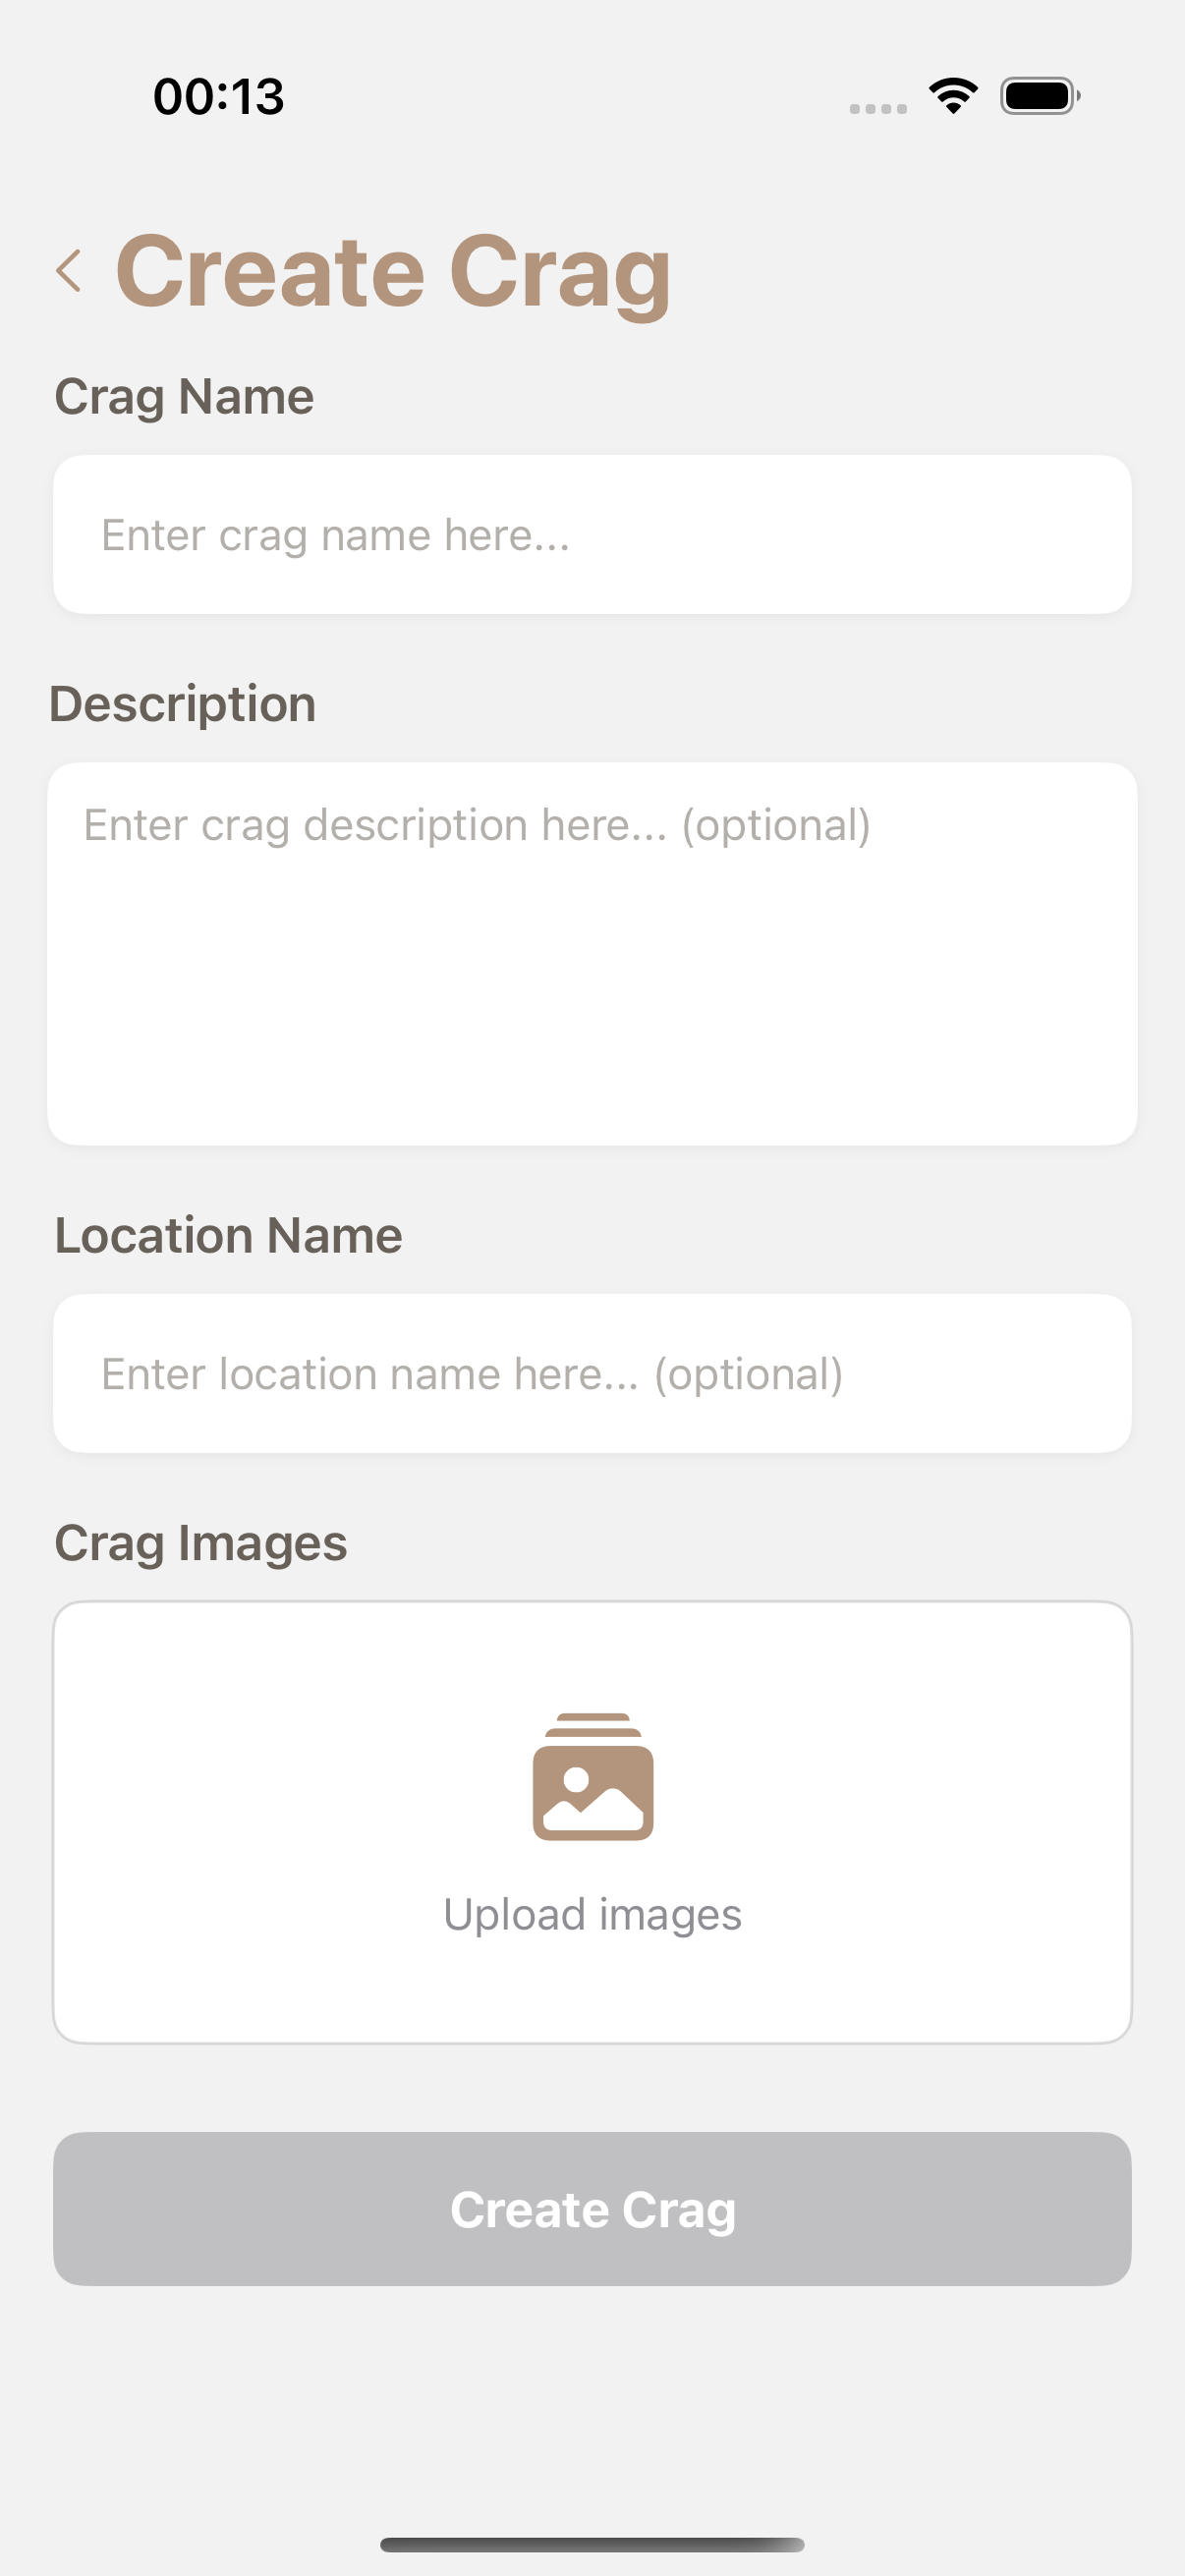
\includegraphics[width=\textwidth]{images/implementacija/editing-options/create_crag.png}
        \caption{Mobilna aplikacija}
        \label{fig:dodavanje_lokacije_mob}
    \end{subfigure}
    \hfill
    \begin{subfigure}[b]{0.6\textwidth}
        \centering
        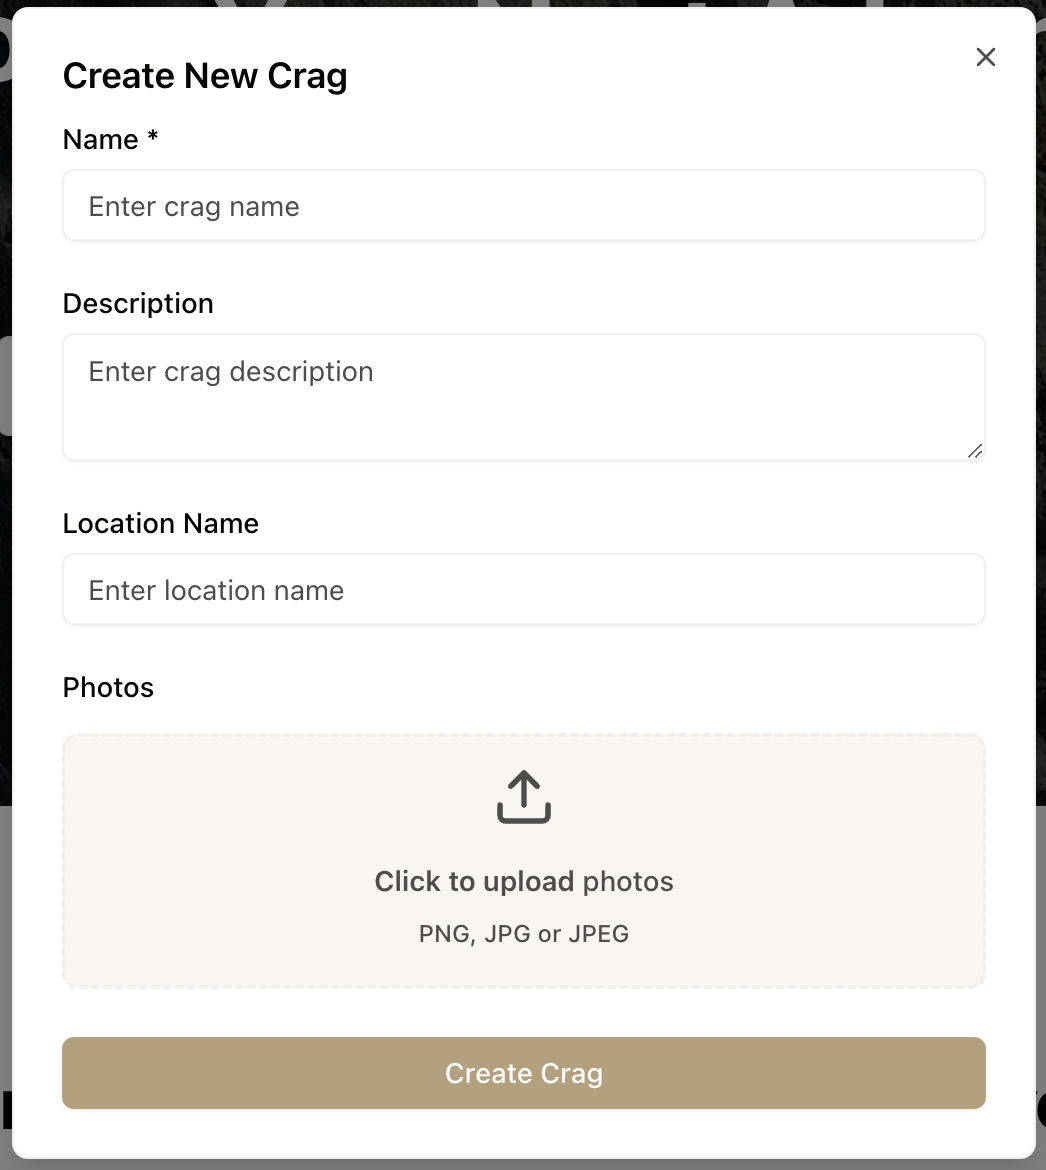
\includegraphics[width=\textwidth]{images/implementacija/web/editing-options/create-crag.png}
        \caption{Web aplikacija}
        \label{fig:dodavanje_lokacije_web}
    \end{subfigure}
    \caption{Dodavanje nove penjačke lokacije}
    \label{fig:dodavanje_lokacije}
\end{figure}

Ovlašteni korisnik odabirom ove opcije pristupa formi za unos nove penjačke lokacije (slika~\ref{fig:dodavanje_lokacije}). Potrebno je unijeti naziv penjačke lokacije, opcionalni opis koji može sadržavati informacije o povijesti regije ili slične zanimljivosti, te naziv šire geografske lokacije. Ime geografske lokacije korisnik može samostalno dodati, no ako ne postoji, aplikacija će automatski dodati naziv geografske lokacije na temelju lokacije penjačke lokacije. Ključno, korisnik može dodati jednu ili više fotografija koje vizualno predstavljaju penjačku lokaciju. Nakon unosa svih podataka, nova penjačka lokacija se stvara u sustavu i postaje dostupna svim korisnicima.

\begin{figure}[H]
    \centering
    \begin{subfigure}[b]{0.36\textwidth}
        \centering
        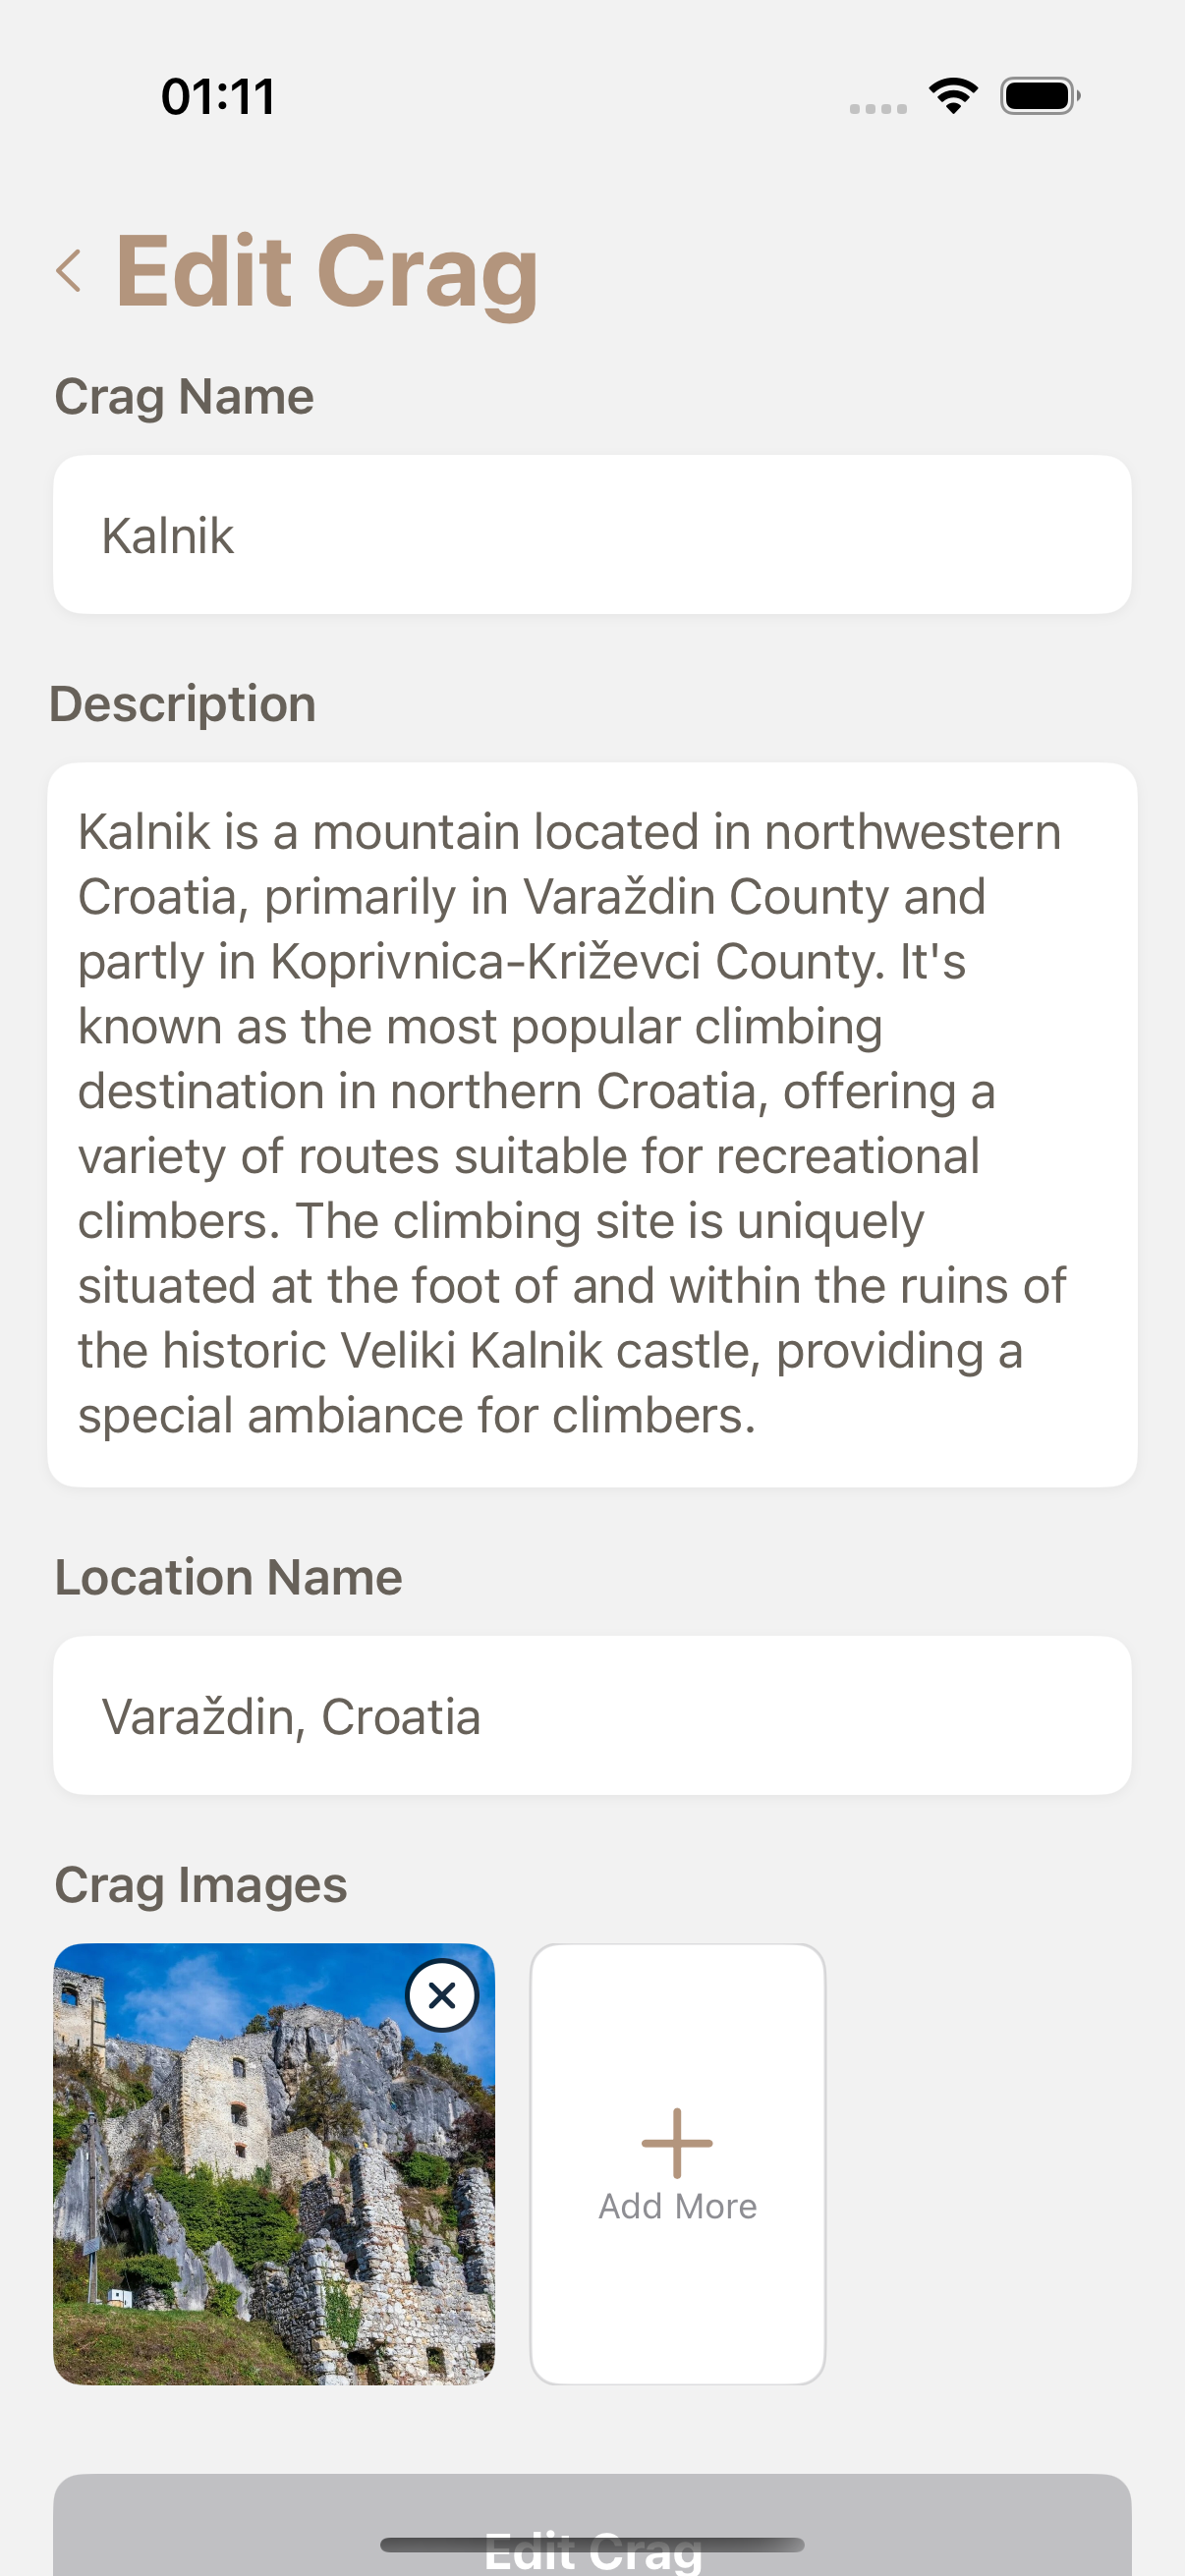
\includegraphics[width=\textwidth]{images/implementacija/editing-options/edit-crag.png}
        \caption{Mobilna aplikacija}
        \label{fig:uredjivanje_lokacije_mob}
    \end{subfigure}
    \hfill
    \begin{subfigure}[b]{0.47\textwidth}
        \centering
        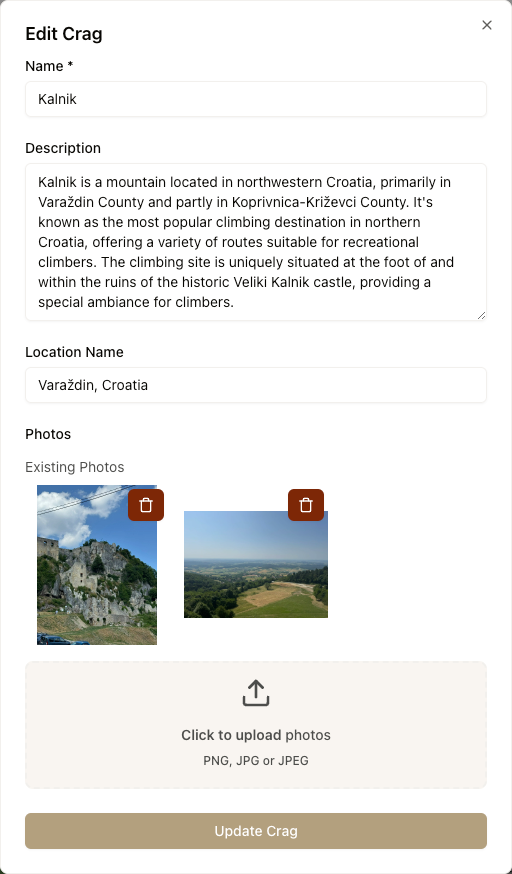
\includegraphics[width=\textwidth]{images/implementacija/web/editing-options/edit-crag.png}
        \caption{Web aplikacija}
        \label{fig:uredjivanje_lokacije_web}
    \end{subfigure}
    \caption{Uređivanje postojeće penjačke lokacije}
    \label{fig:uredjivanje_lokacije}
\end{figure}

Osim kreiranja novih, ovlašteni korisnici imaju mogućnost i uređivanja postojećih penjačkih lokacija (slika~\ref{fig:uredjivanje_lokacije}). Pristup ovoj funkcionalnosti omogućen je u izborniku na zaslonu s detaljnim pregledom penjačke lokacije. 
Sučelje za uređivanje omogućuje promjenu svih prethodno unesenih podataka, uključujući naziv, opis i naziv geografske lokacije. Korisnici također mogu upravljati galerijom fotografija, dodajući nove ili uklanjajući postojeće slike. 

Brisanje penjačke lokacije dostupno je u izborniku na zaslonu detaljnog pregleda penjačke lokacije. Klikom na opciju "Izbriši penjačku lokaciju" (eng. \textit{Delete crag}) korisniku se prikazuje prozor s upitom o potvrdi brisanja. Ako korisnik potvrdi brisanje, penjačka lokacija se briše iz sustava i postaje nedostupno svim korisnicima.

\subsection{Upravljanje korisničkim ovlastima}

Kako bi se osigurala kontrola nad unosom i uređivanjem podataka, a istovremeno omogućio doprinos više ljudi, sustav implementira mehanizam za upravljanje korisničkim ovlastima na razini pojedine penjačke lokacije. Ovoj funkcionalnosti imaju pristup samo vlasnik penjačke lokacije i administratori sustava putem izbornika na zaslonu s detaljnim pregledom penjačke lokacije. 

\begin{figure}[H]
    \centering
    \begin{subfigure}[b]{0.36\textwidth}
        \centering
        
\includegraphics[width=\textwidth]{images/implementacija/editing-options/manage-users.png}
        \caption{Mobilna aplikacija}
        \label{fig:upravljanje_ovlastima_mob}
    \end{subfigure}
    \hfill
    \begin{subfigure}[b]{0.6\textwidth}
        \centering
        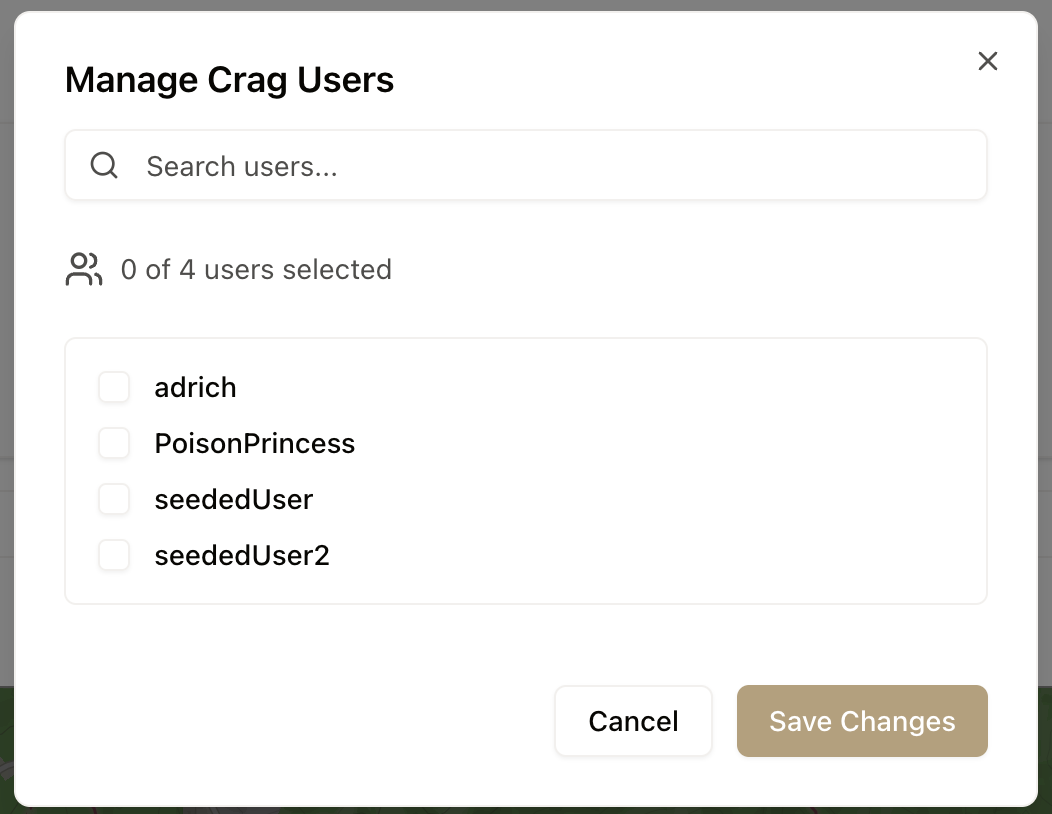
\includegraphics[width=\textwidth]{images/implementacija/web/editing-options/manage-users.png}
        \caption{Web aplikacija}
        \label{fig:upravljanje_ovlastima_web}
    \end{subfigure}
    \caption{Upravljanje korisničkim ovlastima}
    \label{fig:upravljanje_ovlastima}
\end{figure}

Pristupom pregledu za upravljanje ovlastima prikazuje se popis svih korisnika koji trenutno imaju ili mogu dobiti dozvole za uređivanje sadržaja na toj penjačkoj lokaciji (slika~\ref{fig:upravljanje_ovlastima}). Sučelje omogućuje pretragu korisnika po korisničkom imenu te odabir jednog ili više korisnika kojima se žele dodijeliti ili oduzeti ovlasti uređivanja. Time odabrani korisnik dobiva prava uređivanja penjačke lokacije bez davanja potpunih administrativnih ili kreator prava.


\subsection{Dodavanje, uređivanje i brisanje sektora}

Unutar svake penjačke lokacije, ovlašteni korisnici mogu dalje strukturirati sadržaj kreiranjem i uređivanjem sektora. Pristup opciji za dodavanje nalazi se u izborniku na zaslonu s detaljnim pregledom penjačke lokacije. 

\begin{figure}[H]
    \centering
    \begin{subfigure}[b]{0.36\textwidth}
        \centering
        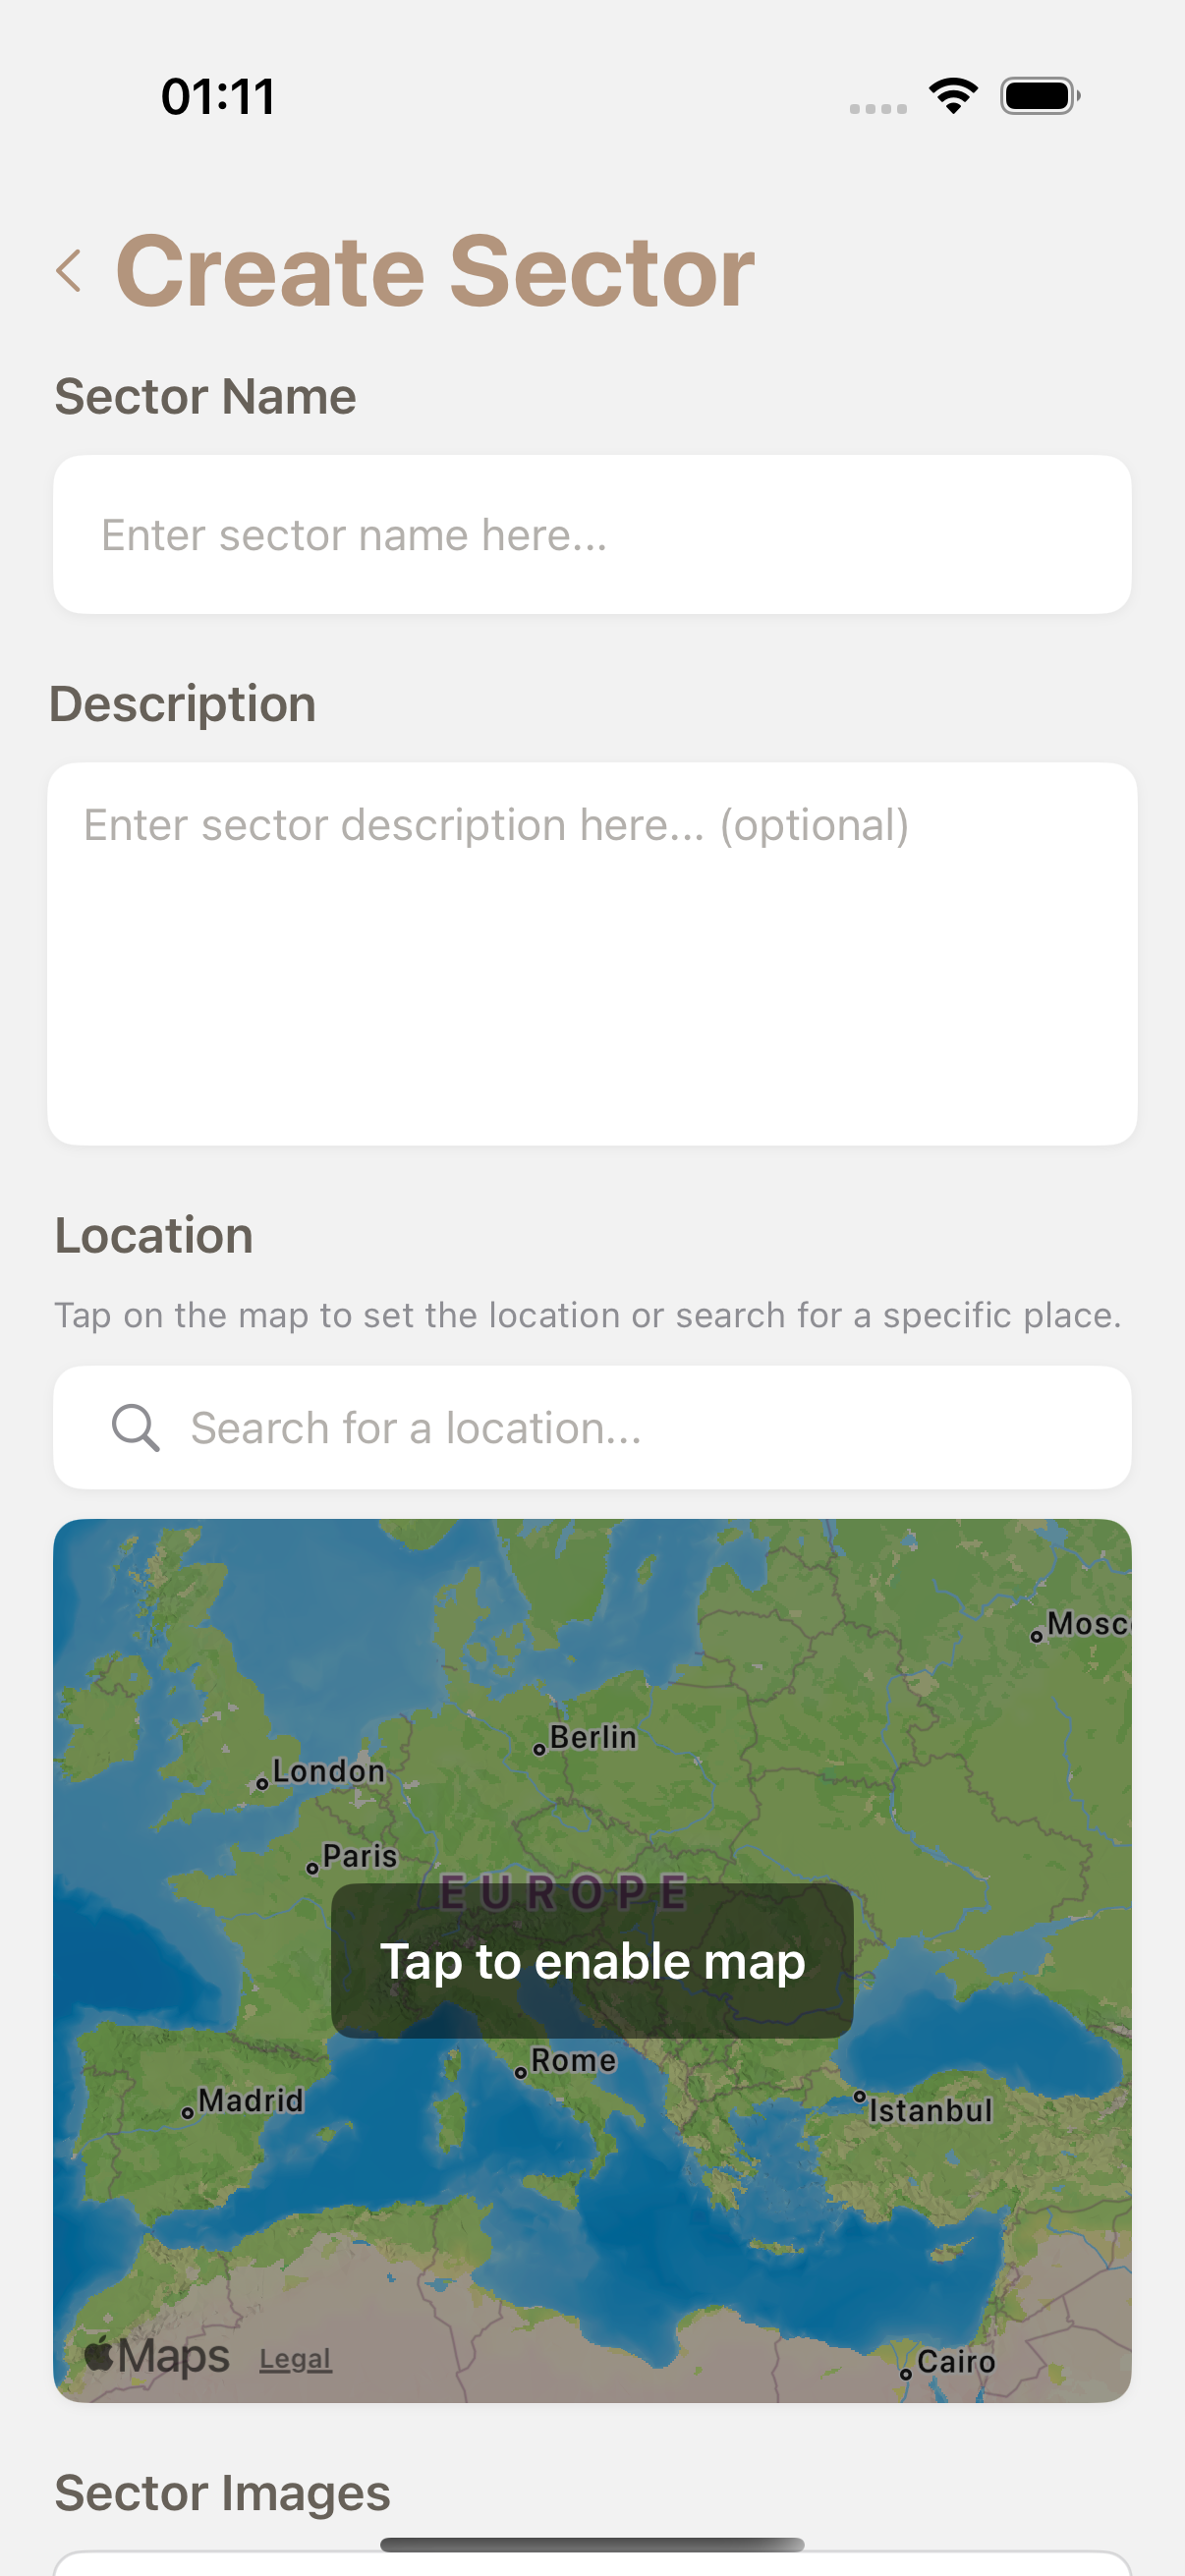
\includegraphics[width=\textwidth]{images/implementacija/editing-options/create-sector.png}
        \caption{Mobilna aplikacija}
        \label{fig:dodavanje_sektora_mob}
    \end{subfigure}
    \hfill
    \begin{subfigure}[b]{0.45\textwidth}
        \centering
        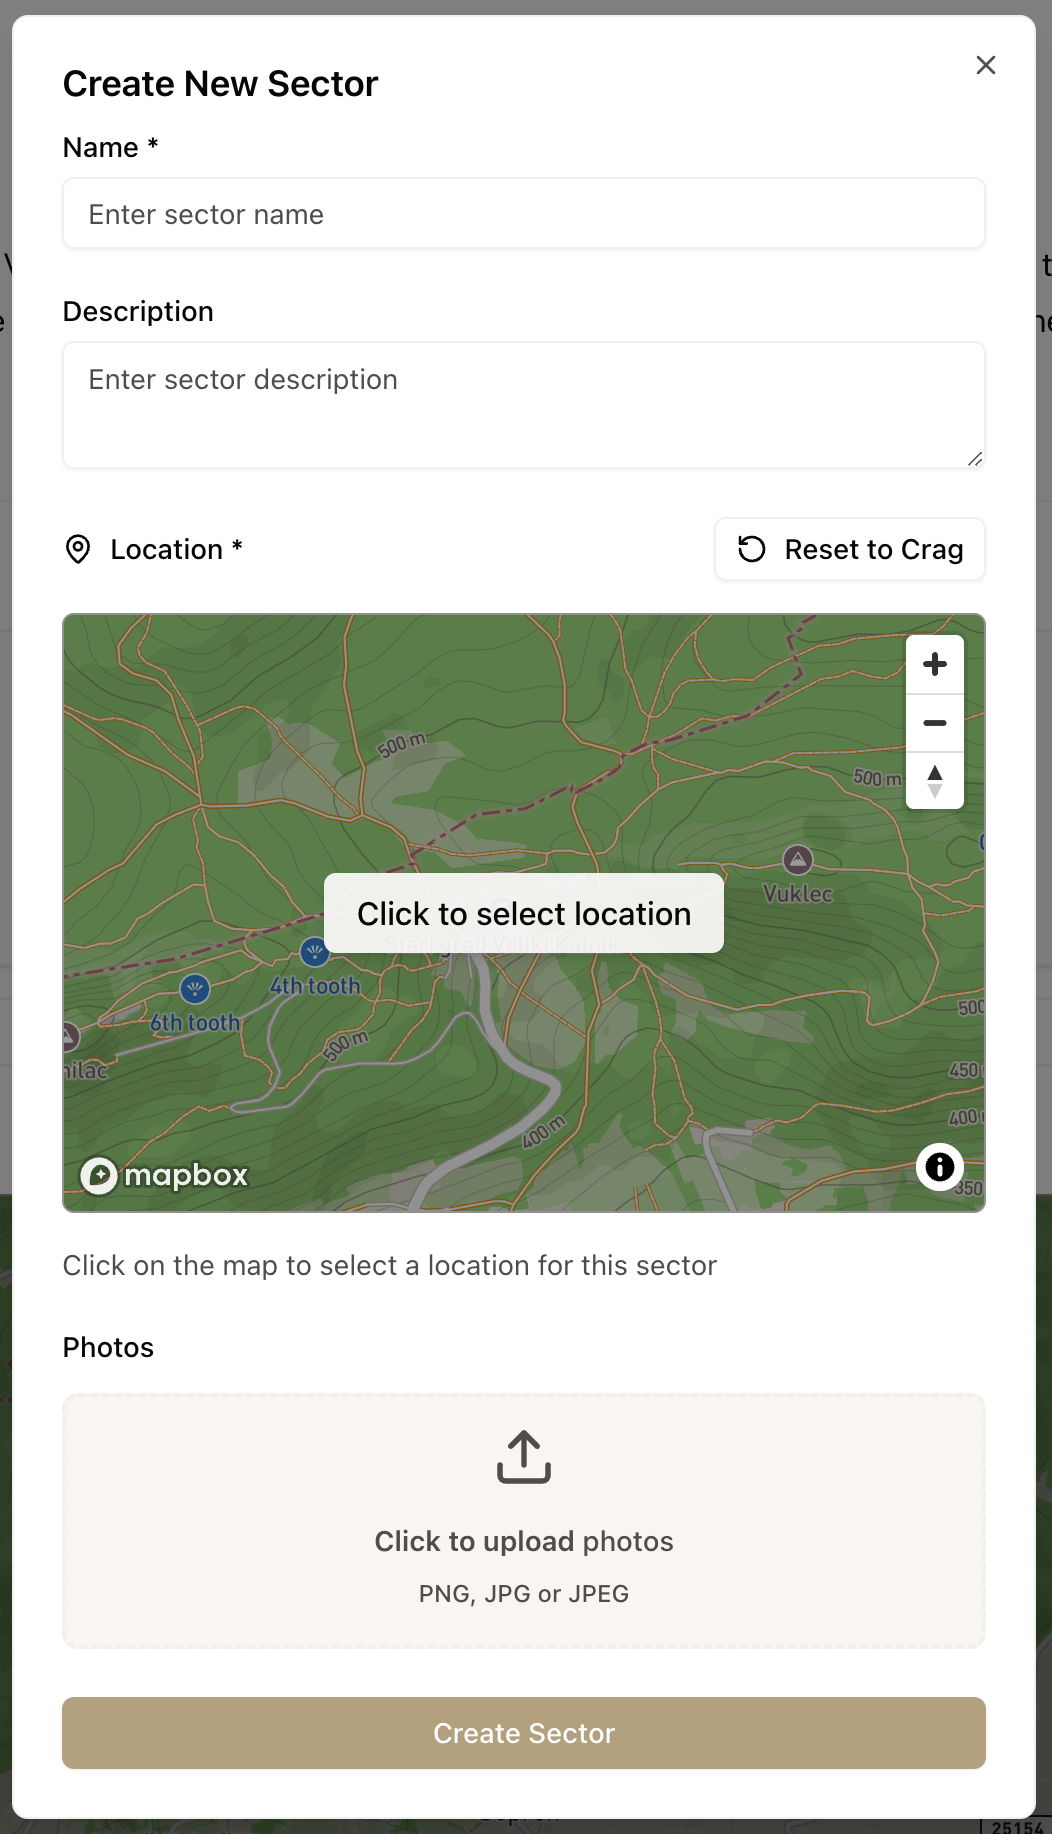
\includegraphics[width=\textwidth]{images/implementacija/web/editing-options/create-sector.png}
        \caption{Web aplikacija}
        \label{fig:dodavanje_sektora_web}
    \end{subfigure}
    \caption{Dodavanje novog sektora}
    \label{fig:dodavanje_sektora}
\end{figure}

Forma za unos novog sektora zahtijeva od korisnika unos naziva sektora i opcionalnog opisa, koji može sadržavati specifične informacije koje su specifične za sektore te ostale relevantne informacije (slika~\ref{fig:dodavanje_sektora}). Osim naziva zahtjeva se i upis lokacije u obliku koordinata. Pregledi taj proces olakšavaju uporabom geografske karte, koja omogućuje korisniku da odabere lokaciju sektora na karti ili pretraživanjem po nazivu lokacije. Kao i kod penjačke lokacije, moguće je dodati jednu ili više fotografija koje vizualno predstavljaju sektor.

Postojeći sektori mogu se uređivati na sličan način. Odabirom određenog sektora, korisniku se prikaže izbornik u kojem se nalazi opcija za uređivanje sektora. Forma omogućuje uređivanje  naziva, opisa, lokaciju i galeriju fotografija. (slika~\ref{fig:uredjivanje_sektora})

\begin{figure}[H]
    \centering
    \begin{subfigure}[b]{0.38\textwidth}
        \centering
        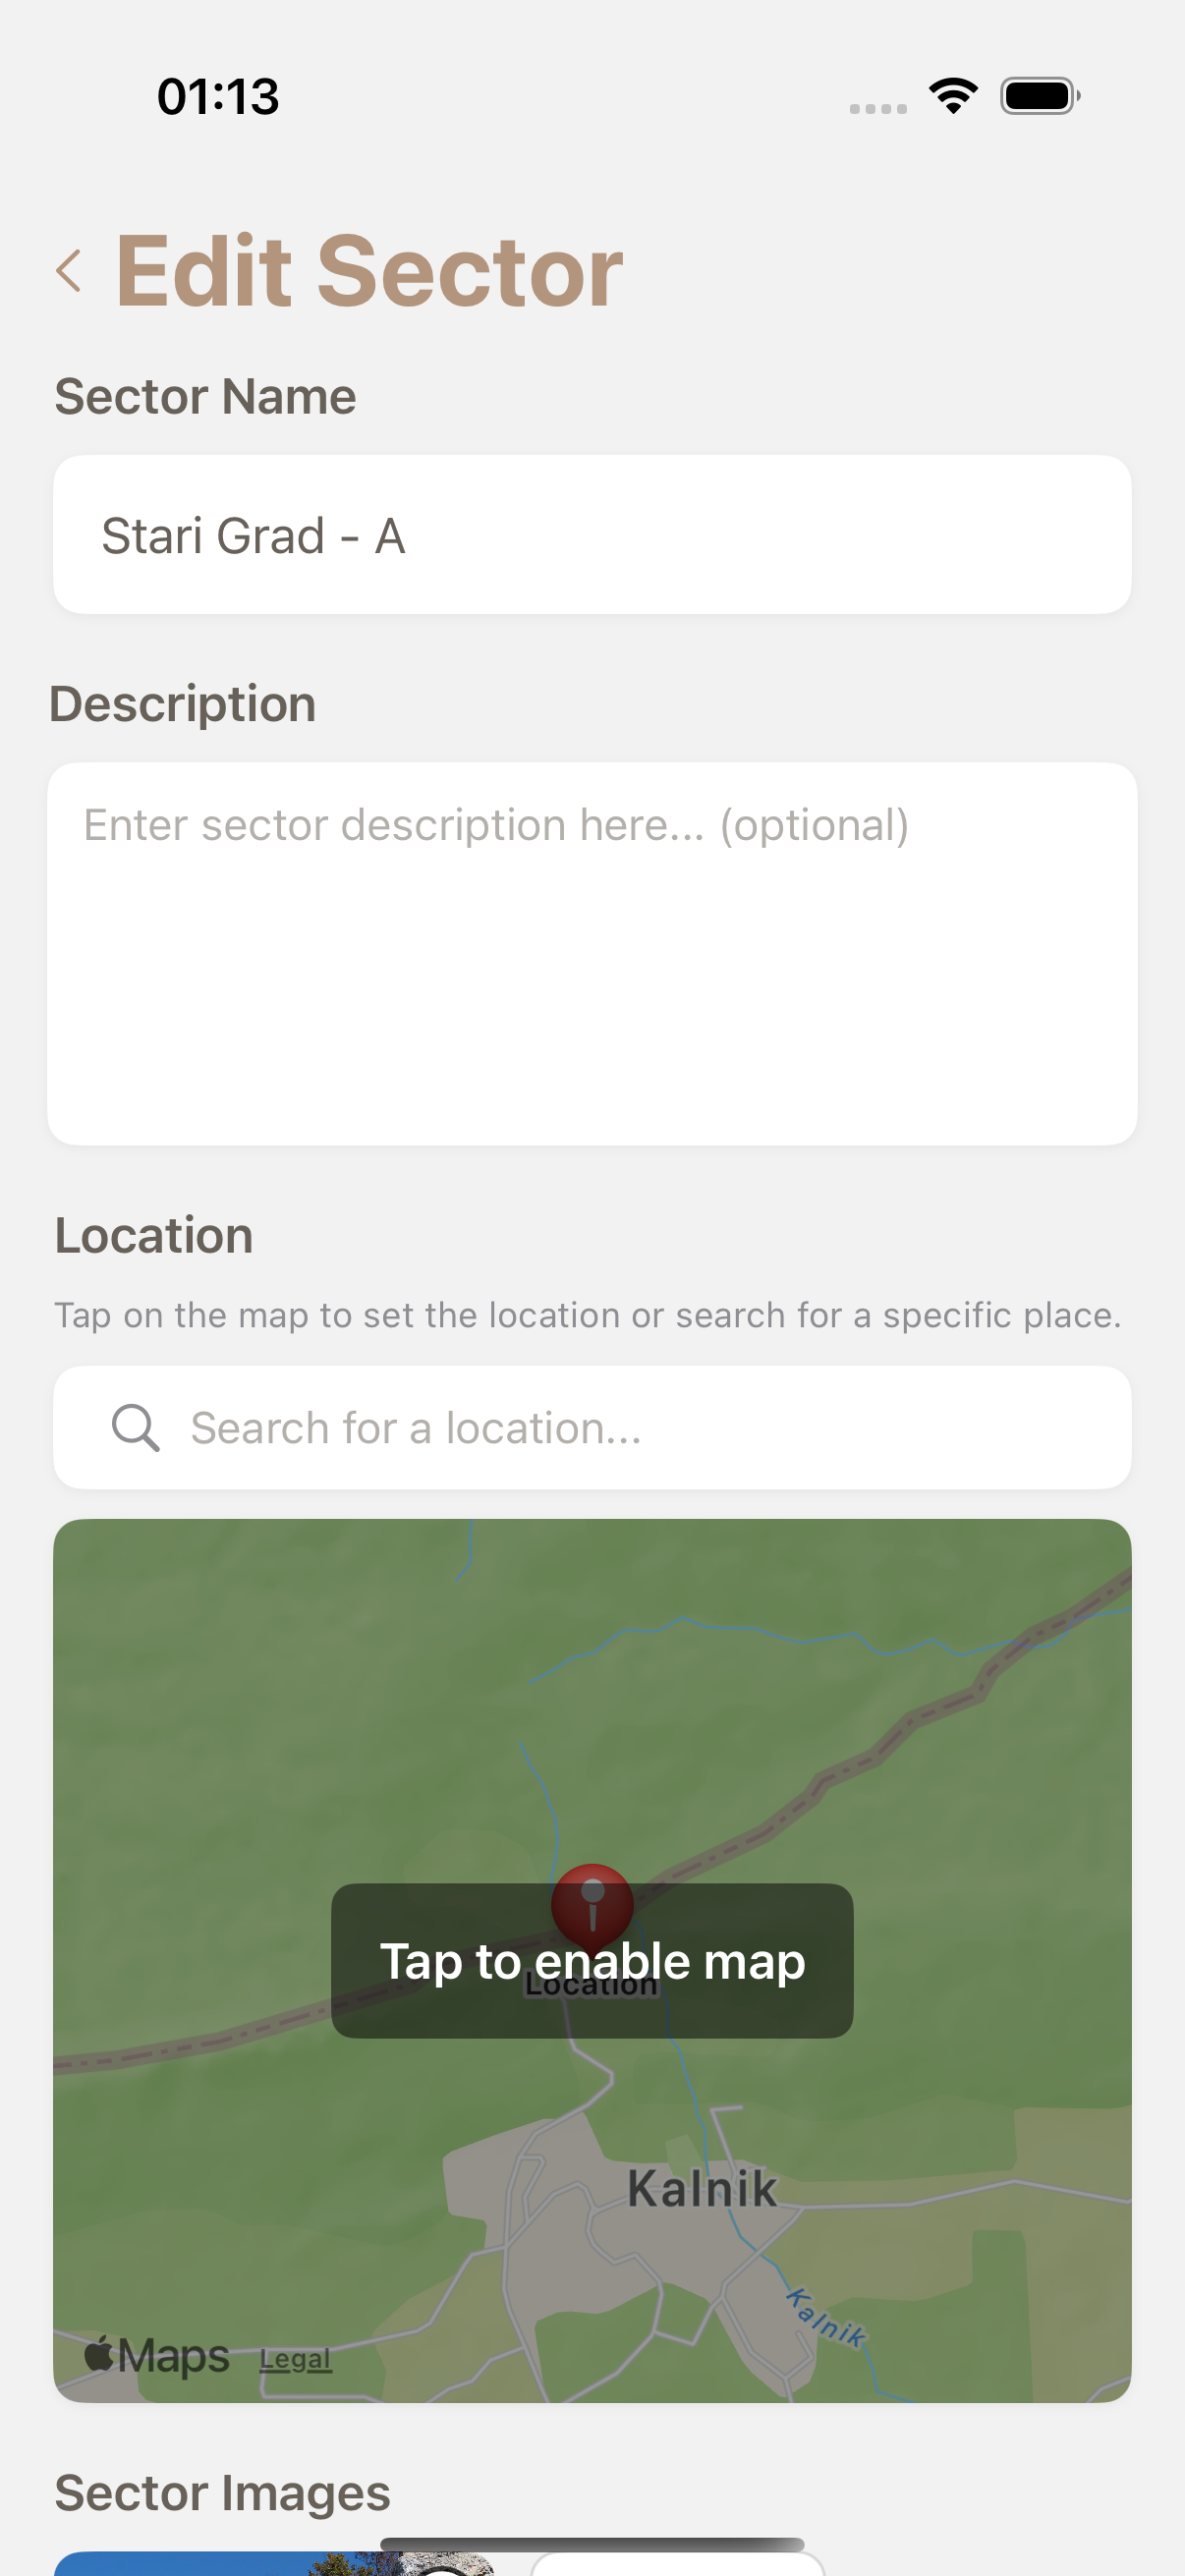
\includegraphics[width=\textwidth]{images/implementacija/editing-options/edit-sector.png}
        \caption{Mobilna aplikacija}
        \label{fig:uredjivanje_sektora_mob}
    \end{subfigure}
    \hfill
    \begin{subfigure}[b]{0.43\textwidth}
        \centering
        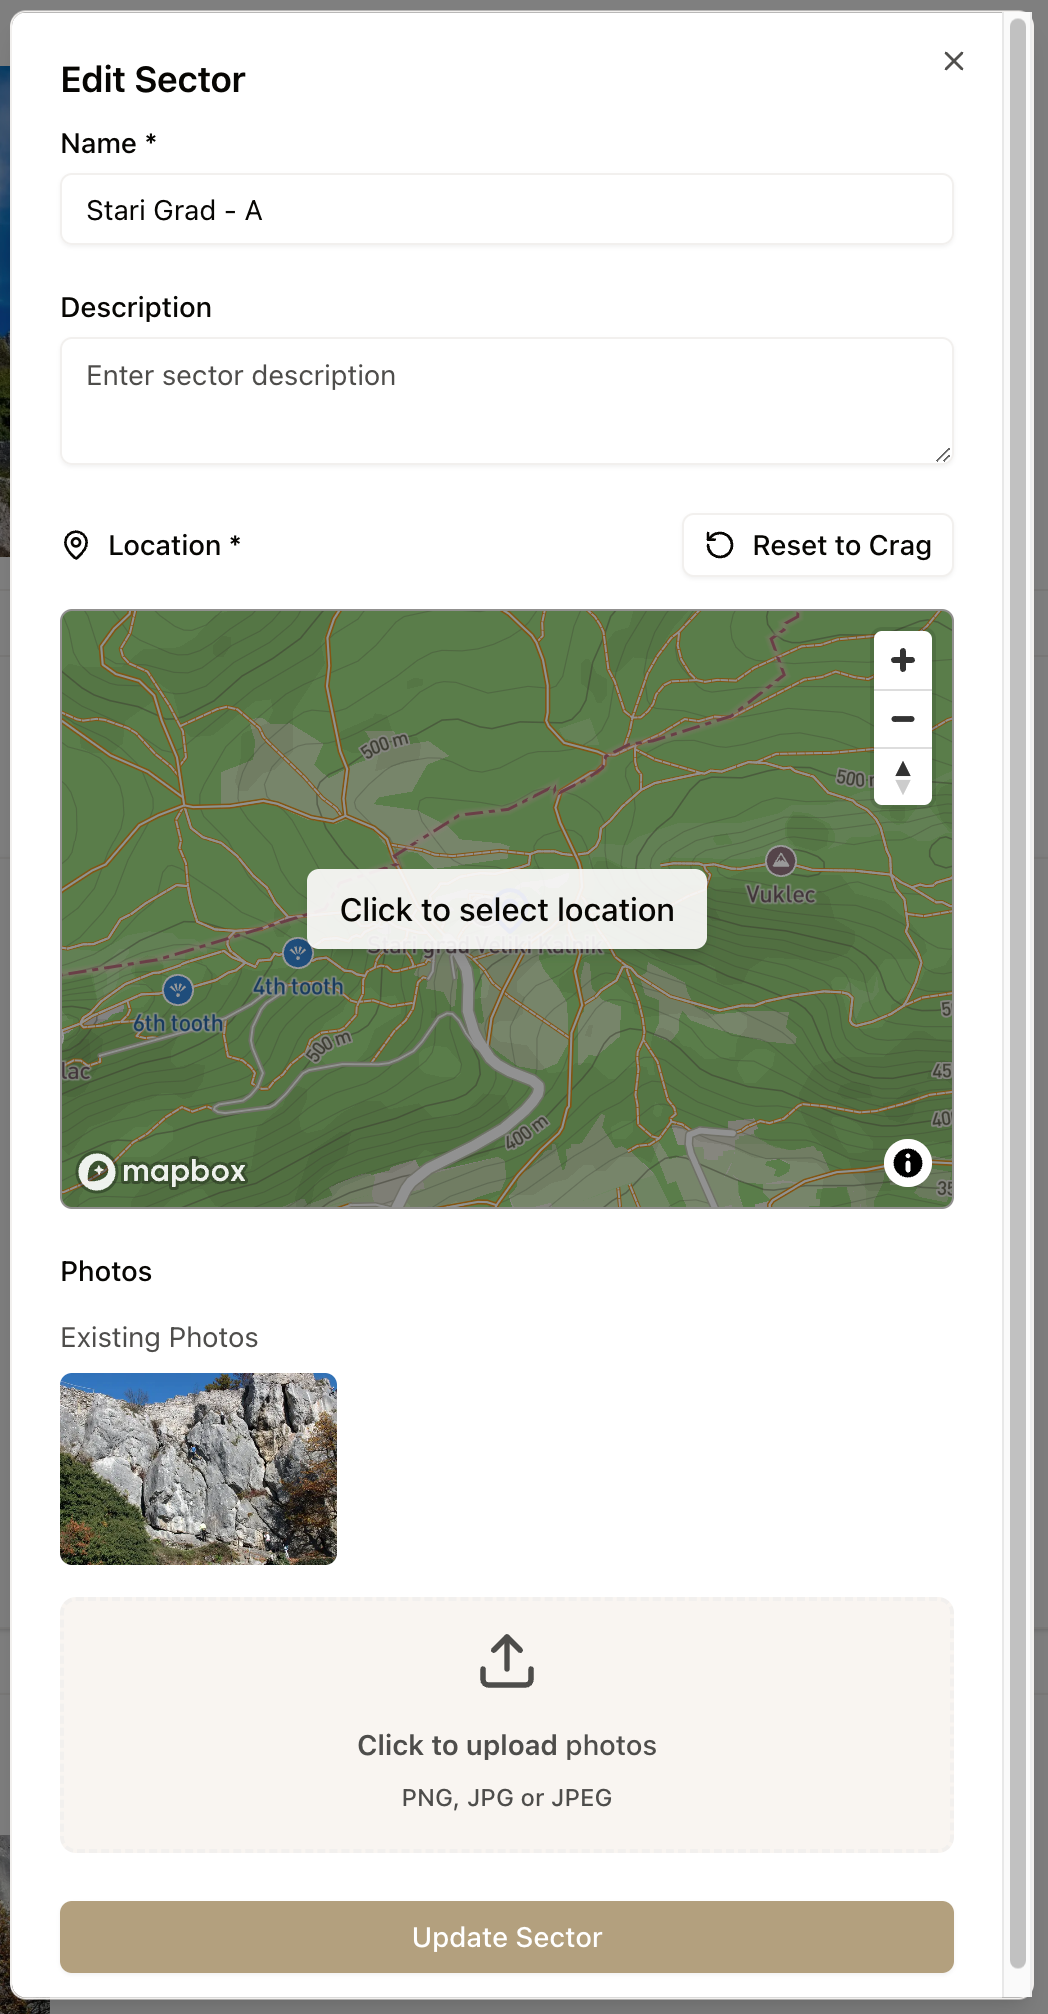
\includegraphics[width=\textwidth]{images/implementacija/web/editing-options/edit-sector.png}
        \caption{Web aplikacija}
        \label{fig:uredjivanje_sektora_web}
    \end{subfigure}
    \caption{Uređivanje postojećeg sektora}
    \label{fig:uredjivanje_sektora}
\end{figure}

Brisanje sektora dostupno je izborniku na zaslonu s detaljnim pregledom penjačke lokacije kada je označen penjački smjer. Klikom na opciju "Izbriši sektor" (eng. \textit{Delete sector}) korisniku se prikazuje prozor s upitom o potvrdi brisanja. Ako korisnik potvrdi brisanje, sektor se briše iz sustava i postaje nedostupno svim korisnicima.


\subsection{Dodavanje, uređivanje i brisanje penjačkih smjerova}

Na najnižoj hijerarhijskoj razini nalazi se unos i uređivanje pojedinačnih penjačkih smjerova. Ovlašteni korisnici mogu dodavati nove penjačke smjerove unutar određenog sektora. Pristup ovoj funkcionalnosti omogućen je u izborniku na zaslonu s detaljnim pregledom penjačke lokacije sa označenim sektorom. 

\begin{figure}[H]
    \centering
    \begin{subfigure}[b]{0.38\textwidth}
        \centering
        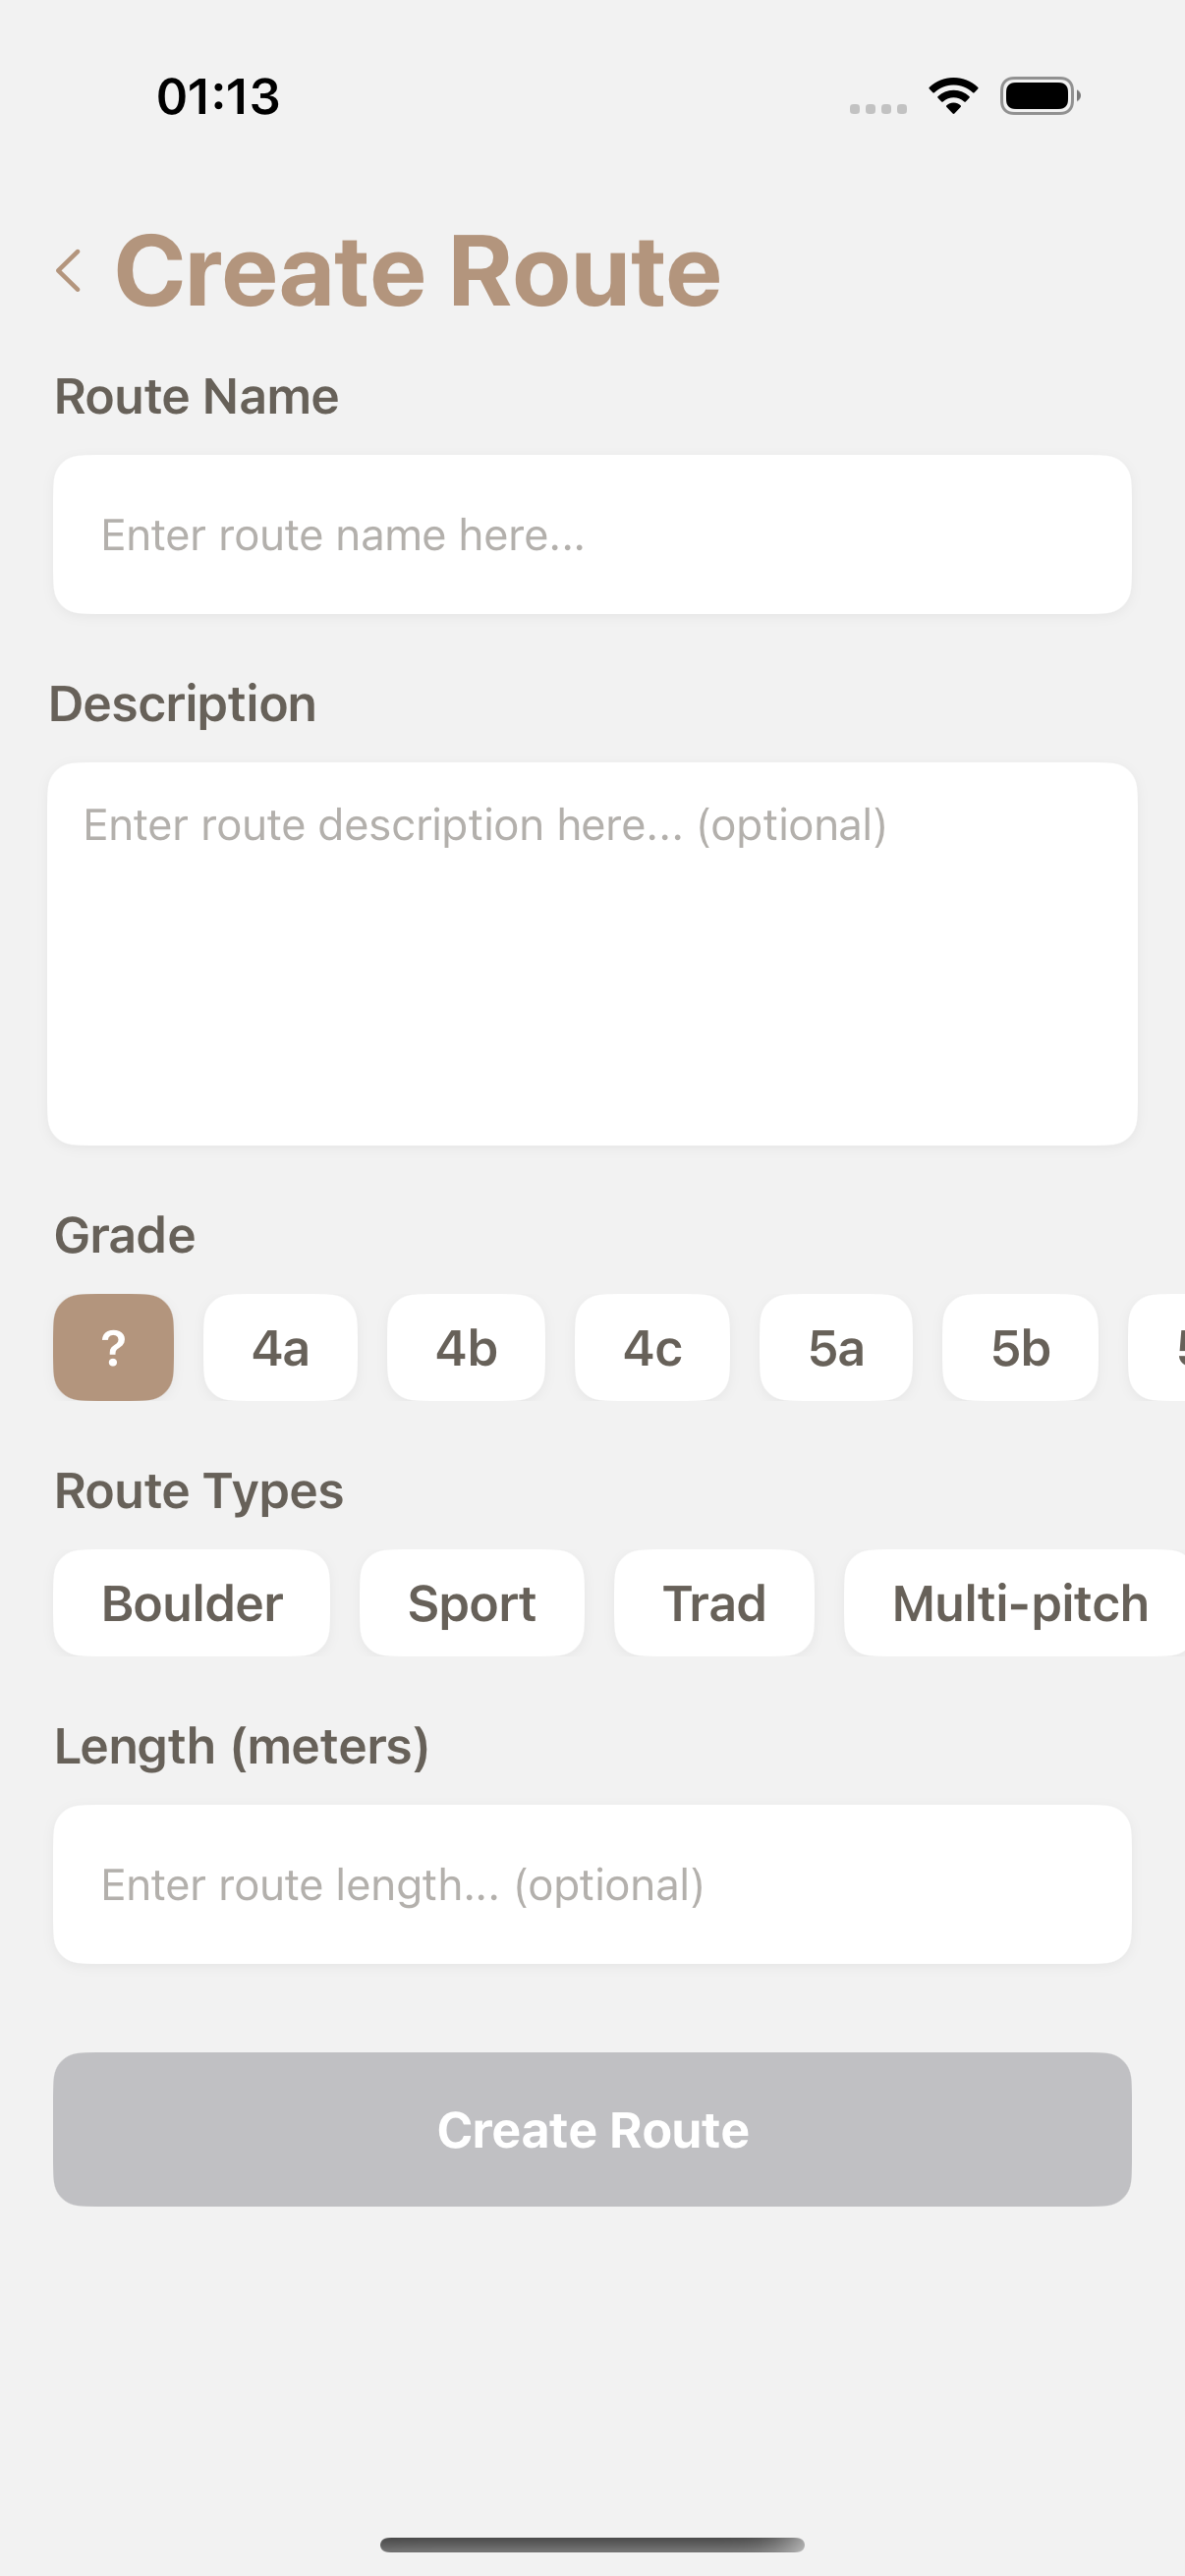
\includegraphics[width=\textwidth]{images/implementacija/editing-options/create-route.png}
        \caption{Mobilna aplikacija}
        \label{fig:dodavanje_smjera_mob}
    \end{subfigure}
    \hfill
    \begin{subfigure}[b]{0.55\textwidth}
        \centering
        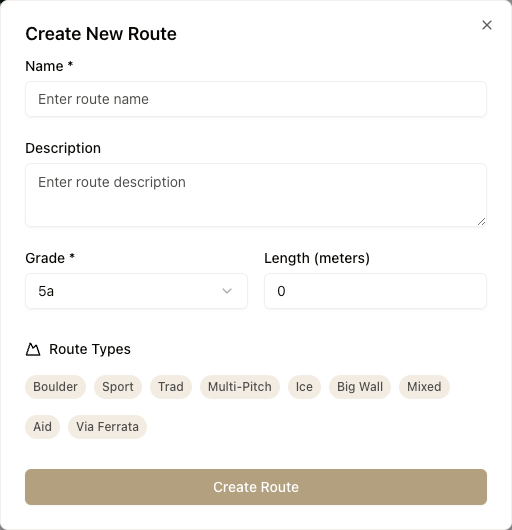
\includegraphics[width=\textwidth]{images/implementacija/web/editing-options/create-route.png}
        \caption{Web aplikacija}
        \label{fig:dodavanje_smjera_web}
    \end{subfigure}
    \caption{Dodavanje novog penjačkog smjera}
    \label{fig:dodavanje_smjera}
\end{figure}

Forma za kreiranje novog penjačkog smjera uključuje polja poput naziva, opisa, težine, tipa penjačkog smjera i dužine (slika~\ref{fig:dodavanje_smjera}). Opcije za tip penjačkog smjera uključuju boulder, sportski, tradicionalni ili smjer s više penjačkih smjerova. 
Važno je primjetiti kako opcija dodavanja slike penjačkog smjera nije dostupna u formi za dodavanje novog penjačkog smjera. Dodavanje fotografije je moguće nakon kreiranja penjačkog smjera u pregledu detalja penjačkog smjera i dostupno je samo na mobilnoj aplikaciji. Klikom na izbornik u gornjem desnom kutu pregleda detalja penjačkog smjera, korisniku se prikazuje izbornik u kojem se nalazi opcija za dodavanje fotografije. Prvi korak u procesu dodavanja fotografije je slikanje penjačkog smjera pomoću kamere mobilnog uređaja. Nakon slikanja, korisniku se prikazuje slika na koju se može ručno ucrtati linija penjačkog smjera. Time je korisnik kreirao referentnu sliku penjačkog smjera koja se može koristiti za prepoznavanje penjačkog smjera (slika~\ref{fig:dodavanje_fotografije_smjera}).

\begin{figure}[H]
    \centering
    \includegraphics[width=0.3\textwidth]{images/implementacija/editing-options/add-route-photo.png}
    \caption{Dodavanje fotografije penjačkog smjera}
    \label{fig:dodavanje_fotografije_smjera}
\end{figure}

Uređivanje postojećeg penjačkog smjera dostupno je u izborniku na zaslonu s detaljnim pregledom tog penjačkog smjera. Na web aplikaciji izbornik se nalazi na izborniku u tablici kada je označen pregled svih sektora ili u listi kada je označen neki sektor. 

\begin{figure}[H]
    \centering
    \begin{subfigure}[b]{0.38\textwidth}
        \centering
        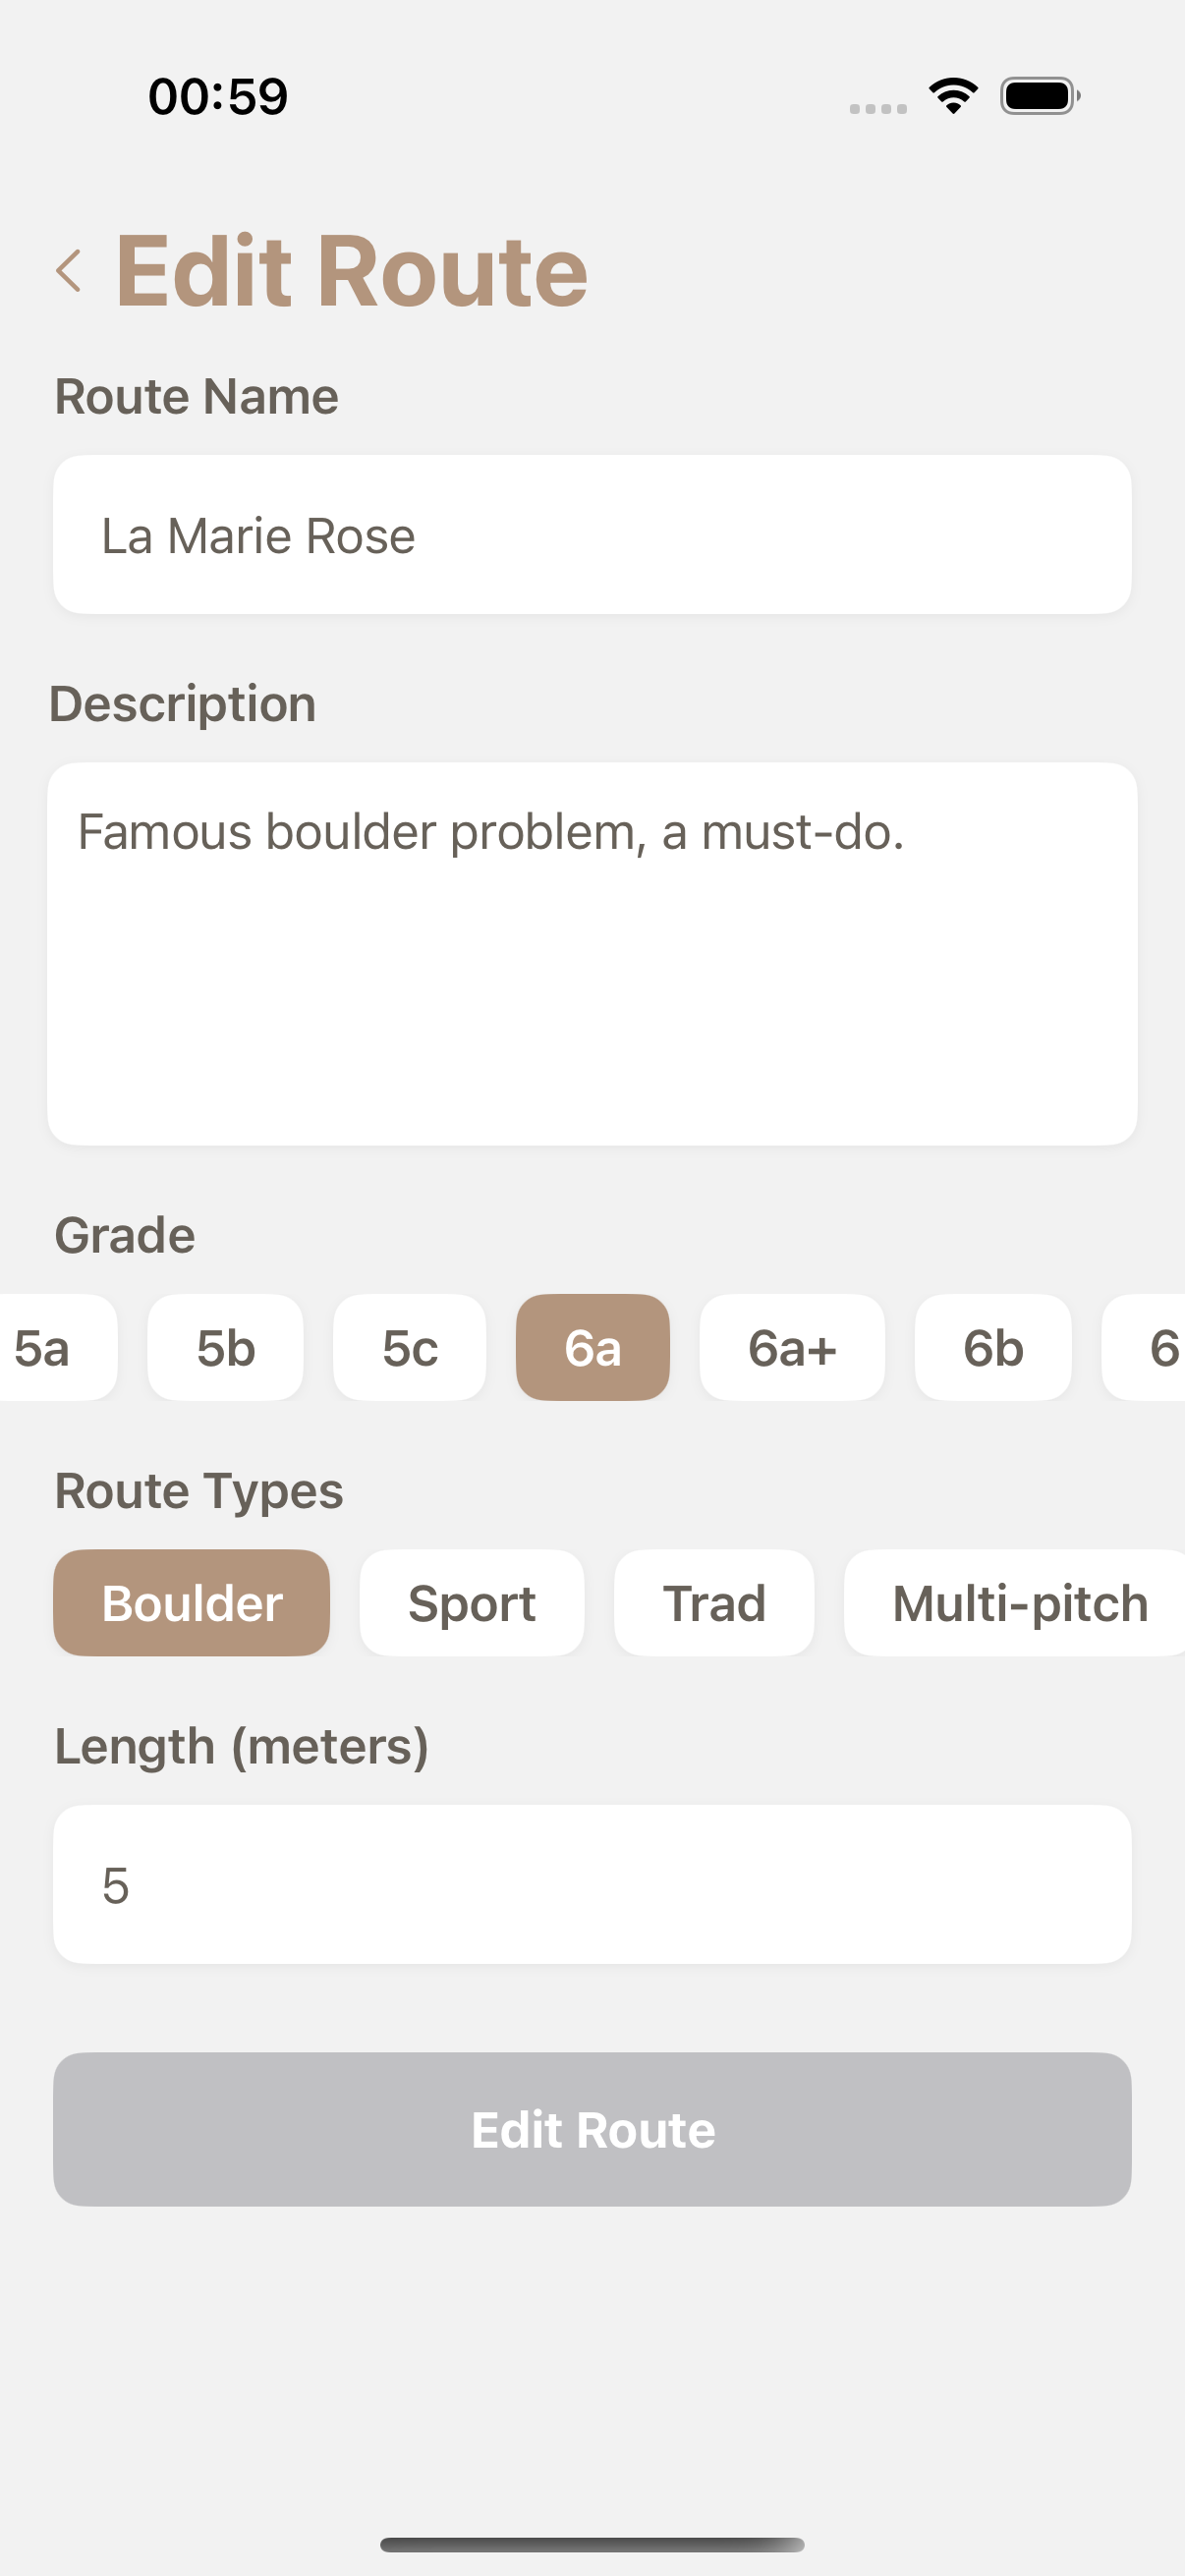
\includegraphics[width=\textwidth]{images/implementacija/editing-options/edit-route.png}
        \caption{Mobilna aplikacija}
        \label{fig:uredjivanje_smjera_mob}
    \end{subfigure}
    \hfill
    \begin{subfigure}[b]{0.55\textwidth}
        \centering
        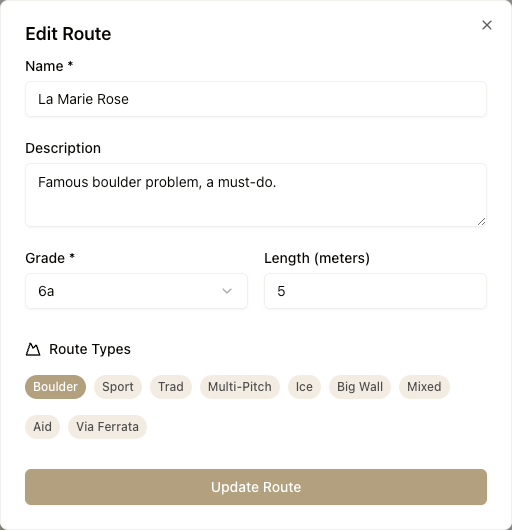
\includegraphics[width=\textwidth]{images/implementacija/web/editing-options/edit-route.png}
        \caption{Web aplikacija}
        \label{fig:uredjivanje_smjera_web}
    \end{subfigure}
    \caption{Uređivanje postojećeg penjačkog smjera}
    \label{fig:uredjivanje_smjera}
\end{figure}

Forma omogućuje uređivanje svih podataka o penjačkom smjeru, uključujući naziv, opis, težinu, tip penjačkog smjera i dužinu, no također je omogućuje brisanje fotografija penjačkog smjera (slika~\ref{fig:uredjivanje_smjera}).


Brisanje penjačkog smjera dostupno je u izborniku na zaslonu s detaljnim pregledom penjačkog smjera. Klikom na opciju "Izbriši smjer" (eng. \textit{Delete route}) korisniku se prikazuje prozor s upitom o potvrdi brisanja. Ako korisnik potvrdi brisanje, penjački smjer se briše iz sustava i postaje nedostupno svim korisnicima.


\subsection{Uređivanje korisničkog profila}

Unutar korisničkog profila, u gornjem desnom kutu, nalazi se izbornik koji sadrži dodatne opcije za upravljanje računom i, ovisno o korisnikovim ovlastima, za doprinos sadržaju aplikacije. Odabirom opcije "Uredi profil" (eng. \textit{Edit profile}) korisnik odlazi na stranicu za uređivanje svojih podataka. Moguće je promijeniti ime, prezime, korisničko ime i datum rođenja. Aplikacija također omogućuje promjenu profilne fotografije te ažuriranje lozinke (slika~\ref{fig:uredjivanje_profila}).

\begin{figure}[H]
    \centering
    \begin{subfigure}[b]{0.35\textwidth}
        \centering
        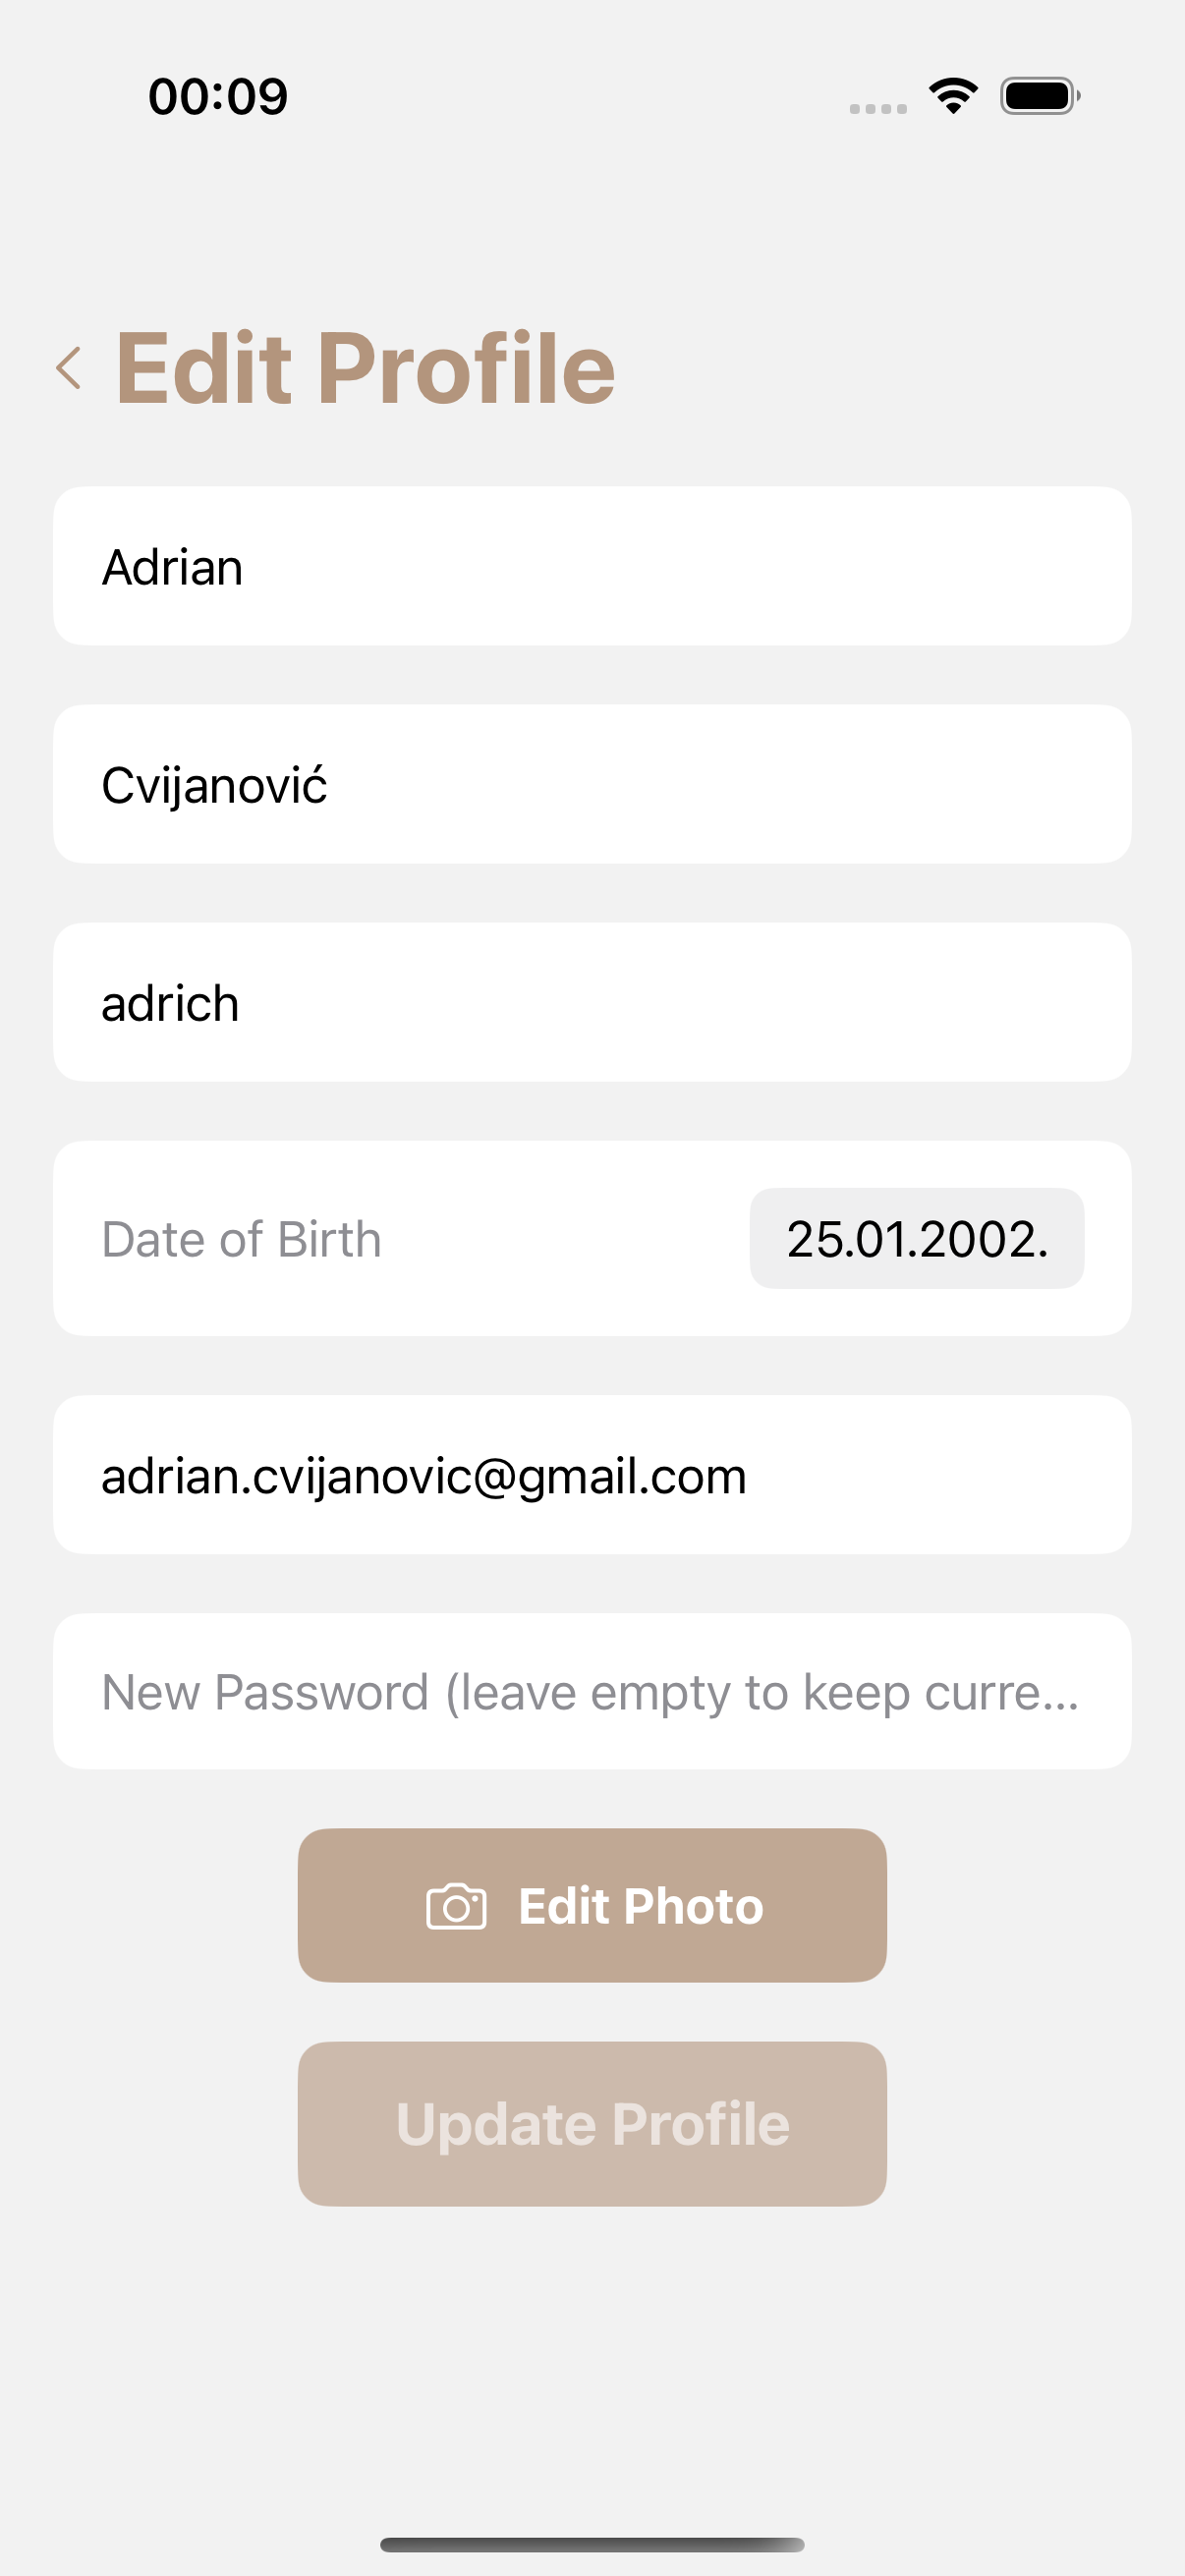
\includegraphics[width=\textwidth]{images/implementacija/editing-options/edit_profile.png}
        \caption{Mobilna aplikacija}
        \label{fig:uredjivanje_profila_mob}
    \end{subfigure}
    \hfill
    \begin{subfigure}[b]{0.55\textwidth}
        \centering
        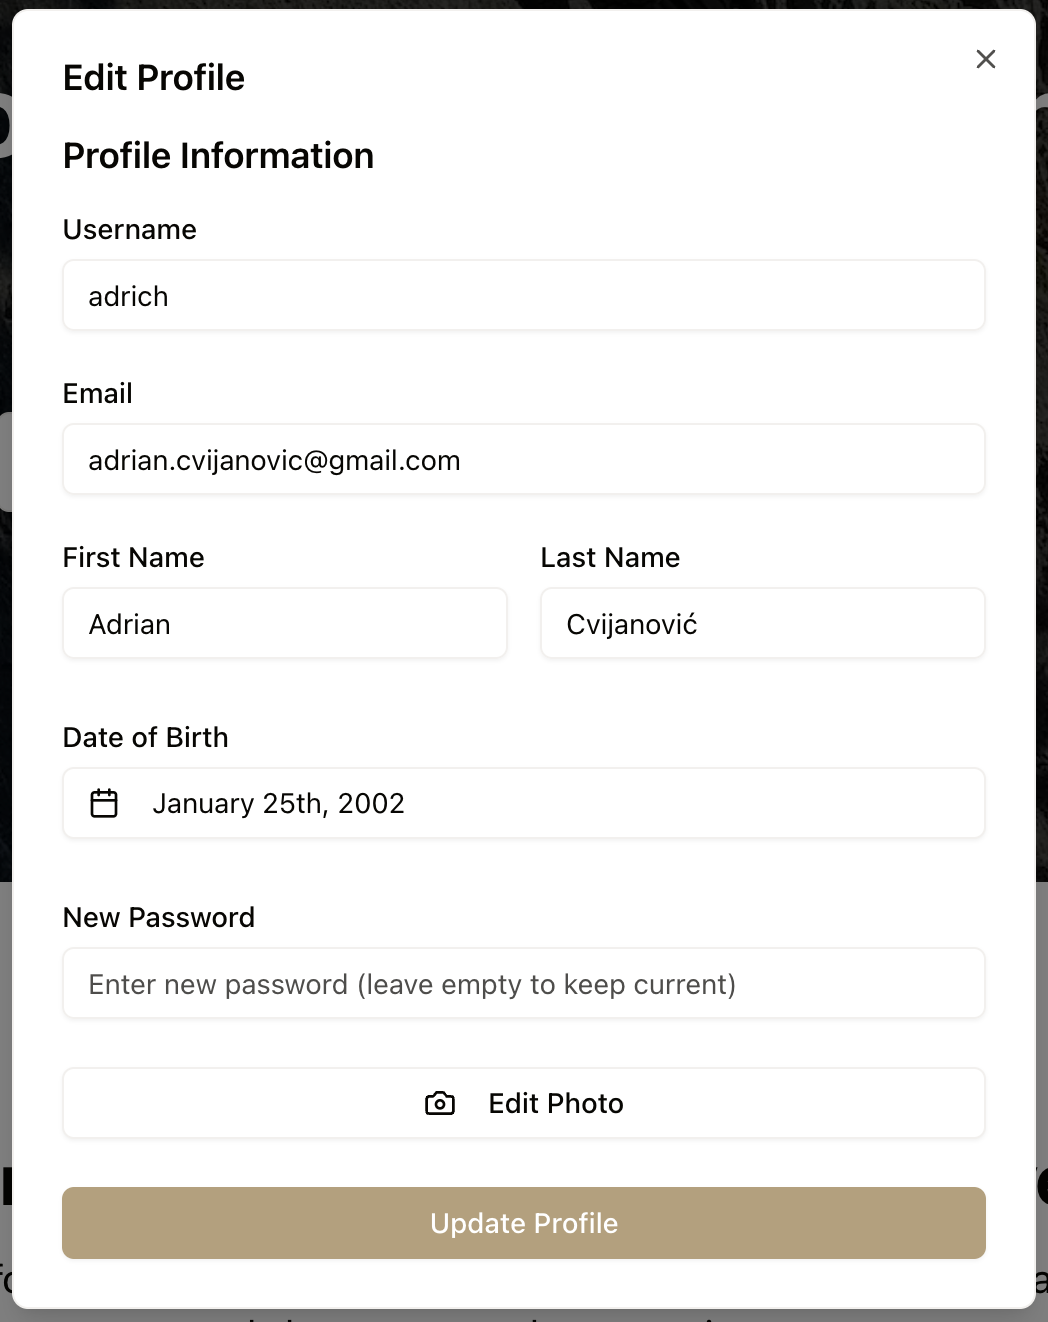
\includegraphics[width=\textwidth]{images/implementacija/web/editing-options/edit-user.png}
        \caption{Web aplikacija}
        \label{fig:uredjivanje_profila_web}
    \end{subfigure}
    \caption{Uređivanje korisničkog profila}
    \label{fig:uredjivanje_profila}
\end{figure}